% !TEX root = main.tex
\renewcommand{\labelenumi}{\alph{enumi})}
\section*{Semanal 7}
\textbf{1. Tomando el siguiente AFN-$\epsilon$, elimina las transiciones epsilon para convertirlo en un AFN.}
\\ 
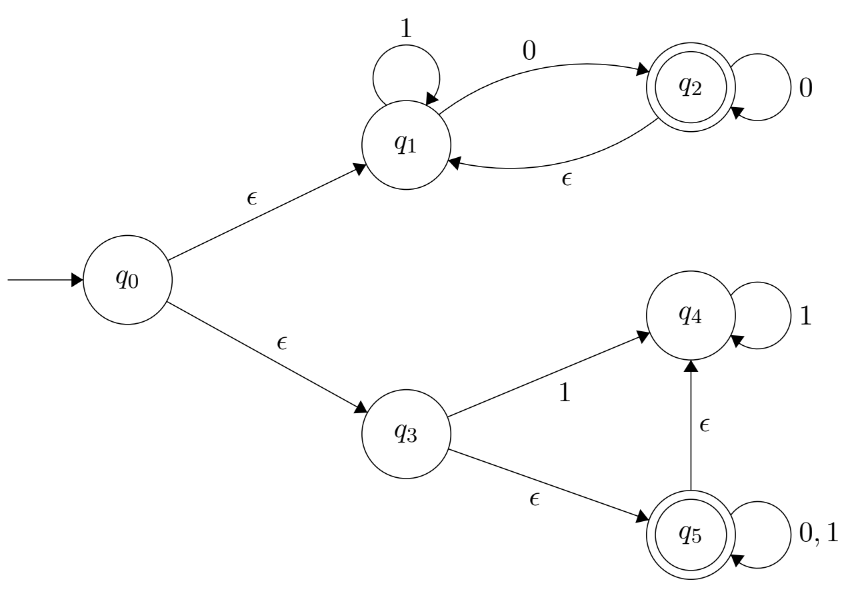
\includegraphics[scale=.50]{AFNe.png}

\begin{center}
    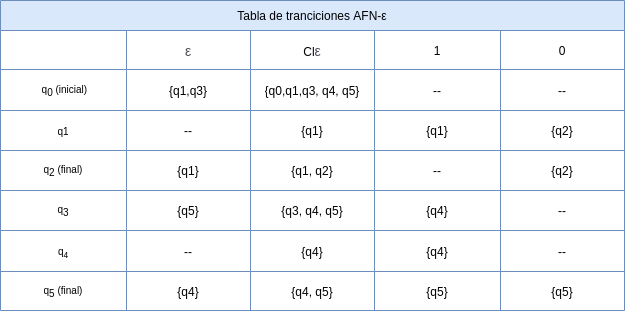
\includegraphics[scale=.50]{firstTable.png}

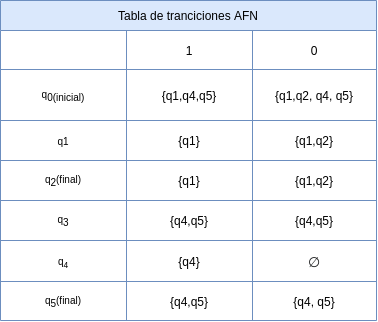
\includegraphics[scale=.50]{secondTable.png}

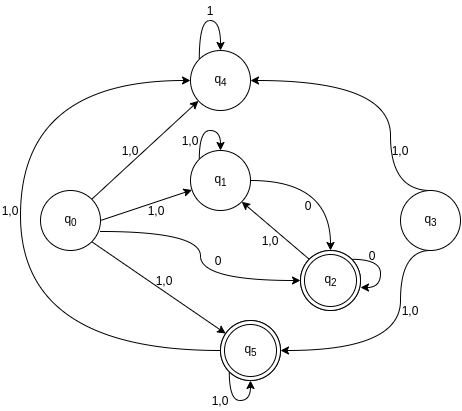
\includegraphics[scale=.50]{automataFN.png}
\end{center}

\textbf{2. Crea un AFN-$\epsilon$ a partir de la siguiente expresi\'on regular:}

\begin{center}
    $c((ab + a)^{*} + (ab + b^{*}))^{*}$

    \begin{equation}
        \underbrace{c}_{\alpha_{0}}\overbrace{(\overbrace{(\underbrace{ab + a}_{\alpha_{1}})^{*}}^{\alpha_{2}} + (\underbrace{ab + \overbrace{b^{*}}^{\alpha_{3}}}_{\alpha_{4}}))^{*}}^{\alpha_{5}}
    \end{equation}

    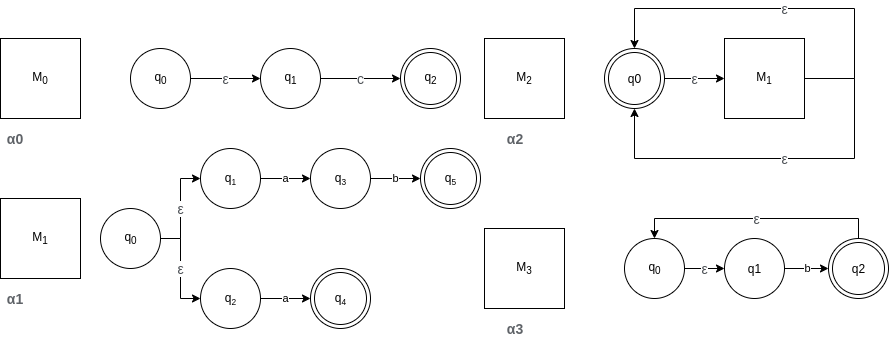
\includegraphics[scale=.50]{machine.png}

    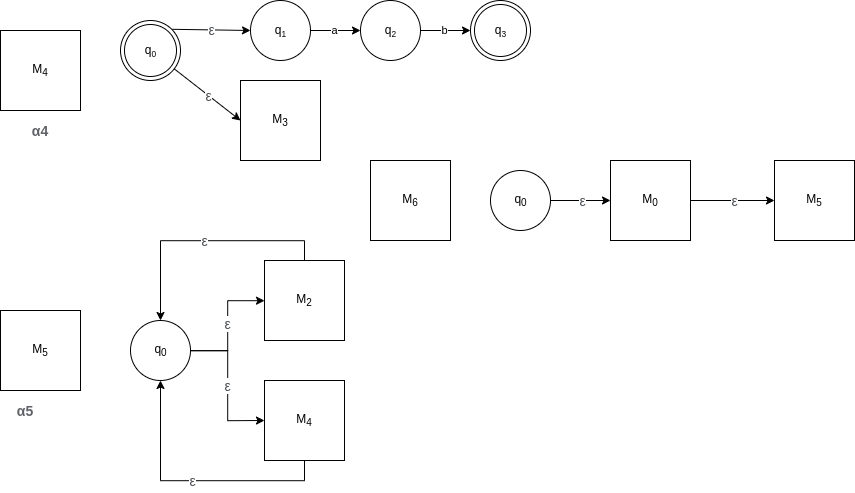
\includegraphics[scale=.50]{machine2.png}

    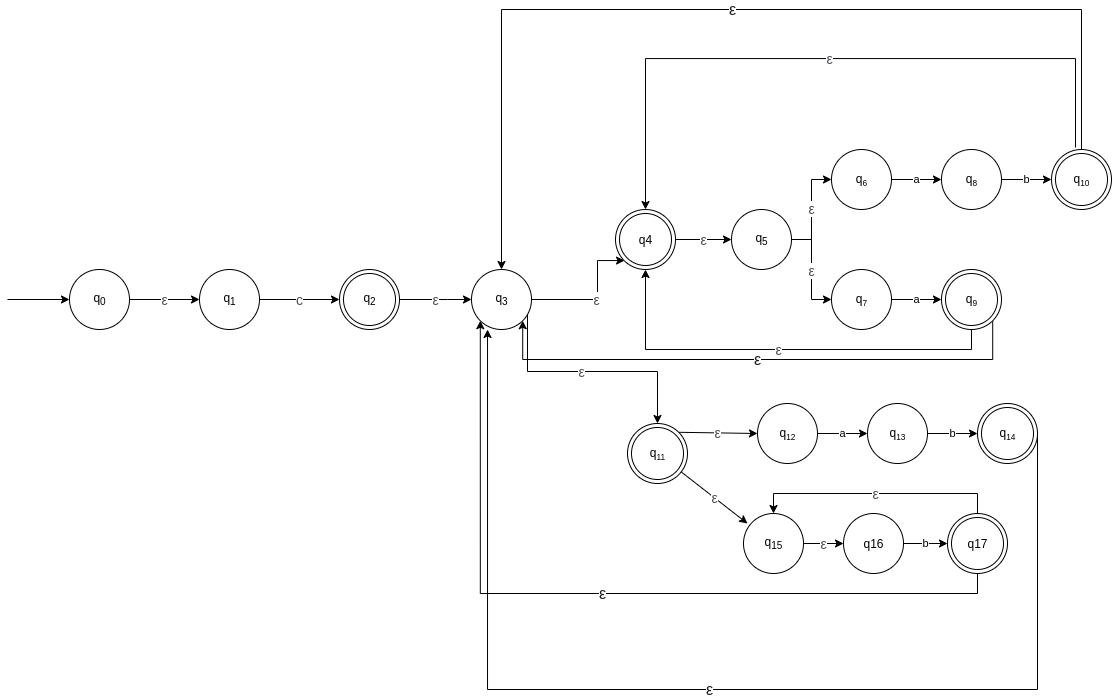
\includegraphics[scale=.50]{automataa.png}

\end{center}


